\chapter{O Projeto}
\label{chapter:projeto}

Os dois últimos capítulos descreveram o conceito de Internet das Coisas e as especificações que o projeto deve contemplar, visando sempre ajudar na construção de sistemas IoT que melhor se encaixem na aplicação. Neste capítulo serão descritos as implementações do projeto, apresentado os motivos das escolhas de tecnologias e protocolos especificados. E terminando sobre persistência de dados em aplicações IoT e por quê a escolha de implementação bancos de dados é importante para a aplicação.


\section{Camada de Abstração}
\label{section:camada_abstracao}

Devido a interação entre dispositivos de aquisição de dados e aplicação e armazenamento de dados, foi necessário uma implementação de um protocolo de comunicação único entre os dispositivos e implementação em cada um destes em suas diferentes linguagens de programação.

O protocolo consiste em uma abstração de um canal de envio de dados chamado Data Stream mostardo em \ref{fig:3.1.0/data_stream}, no qual passam dados após realizar um processamento dos dados em uma determinada velocidade podendo conter um limite de pacote de dados. Nas pontas desse canal estão os Publishers e Subscribers, que serão descritos adiante. Este conceito é uma forma de abstrair, unificar e simplificar a forma de transporte de dados, de uma modo que a interface possa ter o controle sobre os aspectos de transmissão. Cada protocolo na camada de aplicação, implementa este conceito de uma certa forma, porém o desenvolvedor não precisará se preocupar com estes detalhes.

\begin{figure}[h!]

\centering
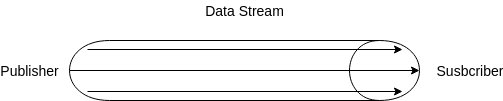
\includegraphics[width=13cm]{./02_Capitulos/02_Cap3/figures/data_stream}
\caption{O conceito de Data Stream para a abstração do transporte de dados}
\label{fig:3.1.0/data_stream}
\end{figure}


\section{Publishers e Subscribers}
\label{section:publishers_subscribers}

Para enviar e receber dados de uma forma a atender os requisitos da seção \ref{section:interface}, foi utilizado um padrão de comunicação recorrente em aplicações contemporâneas, o padrão Publish/Subscribe \cite{amazon:pub_sub}.

O padrão Publish/Subscribe permite que as mensagens sejam transmitidas assíncronas e para vários dispositivos simultaneamente. Para transmitir uma mensagem, um client pode simplesmente enviar uma mensagem para o tópico que os envia imediatamente para todos os subscribers. Todos os componentes que se inscreverem no tópico receberão todas as mensagens transmitidas, a menos que uma política de filtragem de mensagens seja definida pelo assinante.

Qualquer mensagem publicada em um tópico é imediatamente recebida por todos os subscribers do tópico. As mensagens de podem ser usadas para arquiteturas orientadas a eventos ou para desacoplar aplicativos, aumentando  o desempenho, a confiabilidade e a escalabilidade. Com isso, foram criados duas funções possíveis para cada dispositivo dentro deste padrão, os Publishers e os Subscribers, sua comunicação é descrita em \ref{fig:3.2.0/pub_sub}.

\begin{figure}[h!]
\label{fig:3.2.0/pub_sub}
\centering
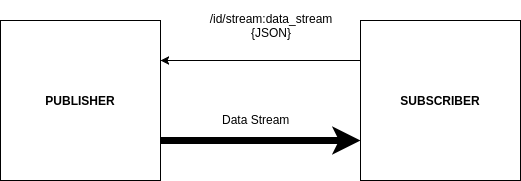
\includegraphics[width=12cm]{./02_Capitulos/02_Cap3/figures/publisher-subscriber_comm}
\caption{Comunicação entre Publishers e Subscribers por Data Stream}
\label{fig:3.2.0/pub_sub}
\end{figure}


Publishers são dispositivos que criam Data Stream  e enviam dados por estes, regulam o processamento dos dados estipulam limites de tamanho de cada pacote de dado e determinam o intervalo de envio de pacotes. O protocolo permite que estes enviem os dados e também permite que outros dispositivos possam passar configurações remotamente para modificar os parâmetros de cada Data Stream, como o intervalo de envio ou outra configuração criada pelo tipo de Data Stream implementado. 

Subscribers estão na outra ponta recebendo os dados, são capazes de enviar as configurações do Data Stream para os Publishers a chegada destes dados como um driver para a aplicação
Essas funcionalidades foram implementadas Orientadas a Objeto e são escaláveis para aplicações mais complexas que serão implementadas para o uso dos sistemas em aplicações de sensoriamento e visualização dos dados.

\section{A implementação}
\label{section:implementacao}

%%% MQTT , Websocket e HTTP %%%


\subsection{MQTT}
\label{subsection:mqtt}

O protocolo MQTT \ref{} foi utilizado escolhido por ser leve e ideal para aplicações em tempo real com vários dispositivos simultaneamente. É um protocolo nos moldes publish/subscribe  ideal para definir a função de cada dispositivo seja enviando dados (Publish) ou recebendo estes (Subscribe).

Para gerenciar os clients (responsáveis pela implementação da comunicação MQTT) em cada dispositivo é necessário um servidor chamado Broker. Este foi implementado com o Mosquitto \ref{}, um broker open source e leve capaz de ser instalado localmente e no servidor do laboratório para testes remotos.